\section{Implementation}\label{s:impl}
\begin{figure*}[t]
    \centering
    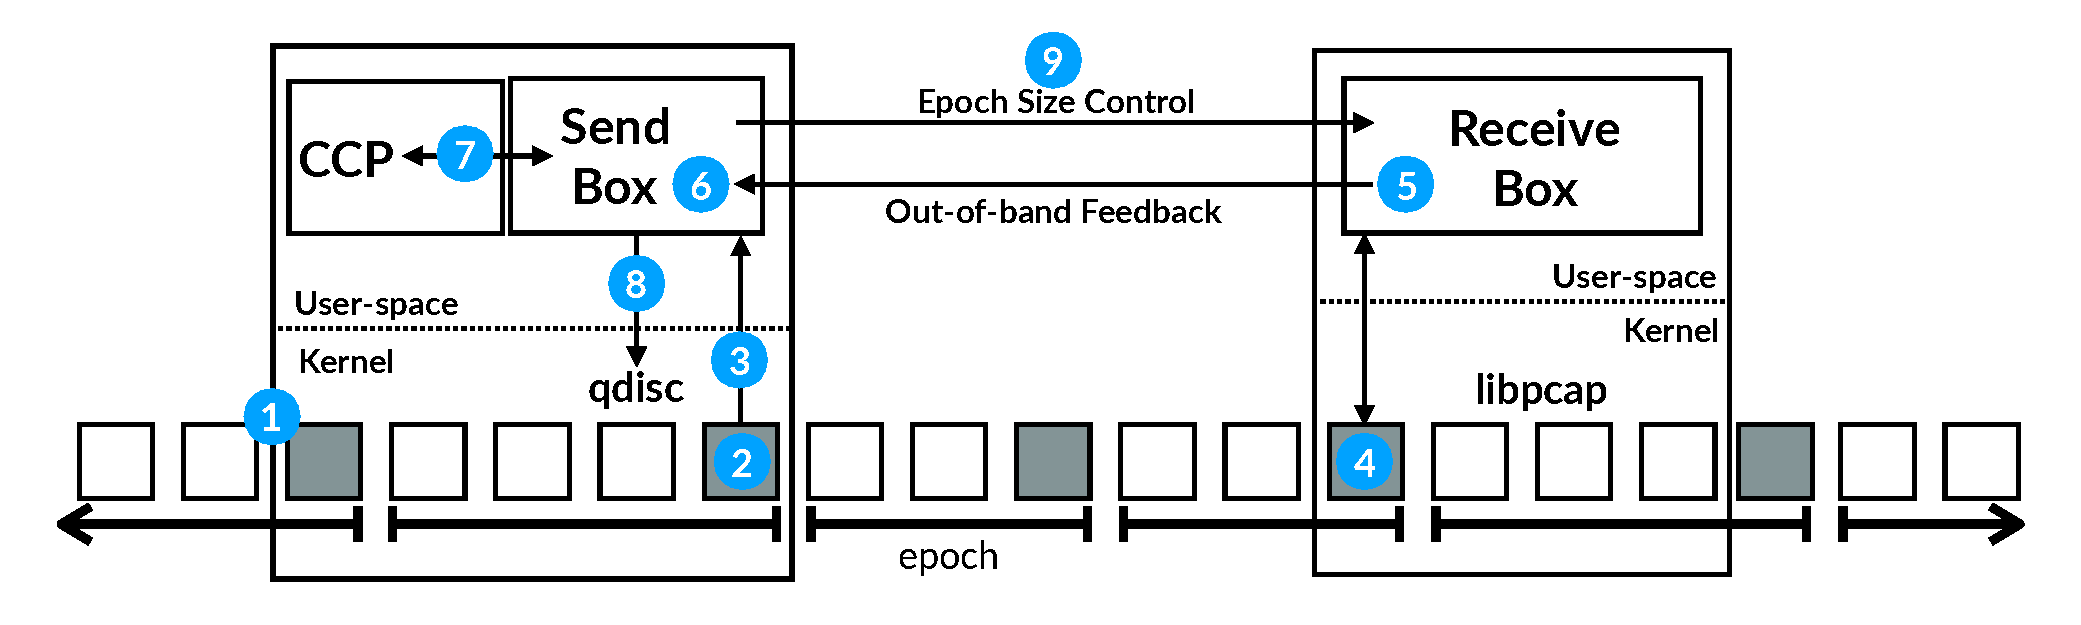
\includegraphics[width=2\columnwidth]{img/bundler-diagram}
    \caption{\name Implementation Overview. Box shading corresponds to the roles described in Figure~\ref{fig:design:block-diag}.}\label{fig:bundler}
\end{figure*}

\name boxes can be implemented as described below (although the specific implementations could vary across deployments).

\Para{\capinbox} It comprises of a \emph{data plane} and a \emph{control plane}. The data plane is responsible for (i) packet forwarding, (ii) tracking the number of sent bytes, (iii) identifying and reporting the epoch boundary packets to the control plane, (iv) enforcing a sending rate (computed by the control plane) on a bundle, and (iv) enforcing the desired scheduling policies for a bundle. It can implemented in software~\cite{bess, click, netbricks, tc}, or in programmable
hardware~\cite{p4}. The control plane, implemented in software, is responsible for (i) measuring congestion signals using the information provided by the data plane along with the feedback from the \outbox, (ii) computing and communicating epoch sizes, and (iii) running the congestion control algorithm for each bundle to compute appropriate sending rates based on the measured congestion signals.

\Para{\capoutbox} It (i) tracks the number of received bytes, (ii) receives and updates epoch size values, (iii) identifies epoch boundary packets and sends feedback message to the \inbox up on receiving one. Similar to \inbox's data plane, it can also be implemented using either software or hardware.

\subsection{Prototype}\label{s:impl:prototype}

We now describe our prototype implementation of the \name boxes.

\Para{\capinbox data plane} We implement it using Linux \texttt{tc}~\cite{tc}.
We patch the TBF queueing discipline (qdisc)~\cite{tbf} to detect epoch boundary packets, and to report them to the control plane using a netlink socket. We use the FNV hash function~\cite{fnv-hash}, a non-cryptographic fast hash function with a low collision rate, to compute the packet content hash for identifying epoch boundaries.
We patch TBF's \texttt{inner\_qdisc} to support SFQ~\cite{sfq}, FQ-CoDel~\cite{fq-codel} and strict prioritization, in addition to the default FIFO. 
By default, TBF instantaneously re-fills the token bucket when the rate is updated; we disable this feature to avoid rate fluctuations caused by our frequent rate updates. 
Our patches to the TBF qdisc comprise $112$ lines of C.

\Para{\capinbox control plane} We implement it to run in user-space in $1167$ lines of Rust.
We use CCP~\cite{ccp} to run different congestion control algorithms (described next). CCP is a platform for expressing congestion control algorithms in an asynchronous format, which makes it a natural choice for our epoch-based measurement architecture. The control plane uses \texttt{libccp}~\cite{ccp} to interface with the congestion control algorithm, and  \texttt{libnl} to communicate with the qdisc.

\Para{Congestion control algorithms} We use existing implementations of congestion control algorithms (namely, Nimbus~\cite{nimbus}, Copa~\cite{copa} and BBR~\cite{bbr}) on CCP to compute sending rates at the \inbox.  If the algorithm uses a congestion window, the \inbox computes an effective rate of $\frac{\text{CWND}}{\text{RTT}}$ and sets it at the qdisc. 
We validated that our implementation of these congestion control schemes at the \inbox closely follows their implementation at an endhost.

%The \inbox also leverages a recently proposed technique~\cite{nimbus} to detect persistent buffer-filling flows. Its basic idea is to use short-timescale pulses to create traffic fluctuations at the bottleneck link, and measure if the cross traffic changes its rate in response to these fluctuations; if it does, it indicates the presence of long-running TCP flows that react to bandwidth variations. When such flows are detected, the \inbox  starts pushing traffic at an increased rate, set to the observed received rate plus a probe factor. Sending faster than the receive rate ensures that the rate of the \inbox eventually exceeds the offered load, thus draining any queue at the \inbox. This, in turn, allows the congestion control algorithms at the unmodified endhosts to compete with the buffer-filling flow, as they would without a \name. The additive probe factor is set in our implementation to one-sixteenth of the maximum receive rate seen so far. 

\Para{\capoutbox} We implement it using \texttt{libpcap} in $188$ lines of Rust. 
%It listens for packets on the interface, checks for epoch packets, and sends the reports to the \inbox. It must maintain per-bundle counters (described in \S\ref{s:impl:discovery}).

\subsection{\name Event Loop}\label{s:impl:loop}
Figure~\ref{fig:bundler} provides an overview of how our \name implementation operates on an already-established bundle.

(1) In the datapath, packets arrive at the \inbox qdisc.
(2) The qdisc determines whether a packet matches the epoch boundary condition (\S\ref{s:measure:marking}). 
If so, it sends a netlink message to the control plane process running in user-space, and then forwards the packet normally (note the datapath does not send packets to user-space). 
(3) The \outbox observes the same epoch boundary packet via \texttt{libpcap}.
(4) It sends an out-of-band UDP message to the \inbox that contains the hash of the packet and its current state. 
(5) The \inbox receives the UDP message, and uses it to calculate the epochs and measurements as described 
in \S\ref{s:measurement}. 
(6) Asynchronously, the \inbox control plane invokes the congestion control algorithm every $10$ms~\cite{ccp}
via \texttt{libccp},
(7) The \inbox control plane communicates the rate, if updated, to the qdisc
using \texttt{libnl}. 
Finally (8), if the \inbox changes the desired epoch length based on new measurements, it communicates this to the \outbox, also out-of-band.
